\chapter{Scientific Problem}
\label{section:scientificProblem}



\section{Problem definition}
\label{section:problemDefinition}

Before defining the proposed solution, we should first illustrate the problem and analyze it in detail. Based on this in-depth analysis, decisions will be made to choose the best fitted approach from a software development perspective.

Software is a vast term generally used to refer to applications, scripts and programs that run on a device. Yet there are different kinds of software, each one having its own challenges and things to be taken into consideration. Designing and implementing an operating system would involve low-level programming and hardware interaction. On the other hand, this becomes absolutely unnecessary if you're developing an eCommerce software product. Indeed, there are practices and patterns that could be applied to all kinds of software, but many are relevant for only one particular field. That is why, as a first step, we should describe the main characteristics of the application that will be built and identify under what type of software it fits.

First of all, our application would involve persistent data. The data about documents which is added by the users should be stored for several years, allowing users to access it, filter it, generate data reports and make conclusions based on them.

As it will be used by the majority of the employees rather than a single person, the application should ensure that many people can access the data concurrently without causing errors. This is especially important for web applications which have thousands or millions of users, but even for a smaller application like ours, concurrency should be handled in a way that would exclude integrity problems and assure data consistency.

Then there is the most important part of the application: its business logic. What data should be stored for each document? What input values are considered valid for each field? Who is allowed to view and edit the data? Which functionalities should the app provide? The answer to all this questions can only be found by analyzing the requirements of the client and turning them into business rules that would serve as the functional engine of the application.

Last but not least, the application needs to provide a GUI\footnote{Graphical User Interface} that would present the data to the user. The challenge here would be to design the application keeping in mind that usability is as important as functionality. A software system meant to improve the effectiveness of processes in an organization should also offer effectiveness and efficiency in its usage. To bring users satisfaction from interacting with the app, the GUI must provide all the desired features, yet keep things simple and intuitive.

The identified characteristics are also described in \cite{patternsOfEnterpriseApplicationArchitecture} as aspects that define Enterprise Applications as a software type. Enterprise Applications are software solutions that provide business logic to handle processes of an organisation in a way that would improve efficiency and productivity. Some people think of a large system when hearing the term "Enterprise Application". However it is important to keep in mind that not all enterprise applications are large and the value they bring to the organization does not depend on their size. What is also important to understand is that even an application for a small organization, with a few users and relatively simple logic, needs to be built in such a way that it will be maintainable and extensible. It could happen that in a couple of years the organization would like to add other processes to the app, thus we have to make sure it allows adding new functionality without having to reimplement already existing logic. This can only be achieved by taking into account well-known design patterns qualified for our purpose.



\section{Theoretical foundations}
\label{section:theoreticalFoundations}

In this section of the thesis we will analyze the theoretical foundations that will further help us design and build the application keeping in mind all the challenges that were previously mentioned.


\subsection{Why a Web distributed system?}
\label{subsection:whyAWebDistributedSystem}

A first and important decision we have to make is whether to develop a desktop application or a web-based one. Indeed, a traditional desktop app doesn't need constant Internet connection in order to be used. It could do all of it's processing on the locally installed app and only sync data with the database once in a while when it has Internet connection. However, this seems to be its biggest and only advantage. Web applications, on the other hand, have a wide range of advantages. To start with, a web application runs on a web browser, which means there is no need to install additional software on the computer. This makes it accessible from a wide range of devices and operating systems. In addition, it gives users freedom to access the app from anywhere, anytime, via any device with an Internet connection, allowing them to solve urgent tasks without a trip to the office. App maintainance is also less complicated - once an update is made on the host server, users can access it without manual updates on their computer. These are the main reasons why building a web application was chosen over a classical desktop one.

% think about the title?
\subsection{Layer architecture}
\label{subsection:layerArchitecture}

A web application architecture is based on a \textit{client-server} model, which is a distributed application system that divides tasks between the server - the provider of resources, and the client, which communicates with the server via requests made over the network. As stated in \cite{databaseProgrammingWithJdbcAndJava}, the simplest shape a client-server architecture can take is a \textit{two-tier} architecture. This originated back in the 90s long before the rise of the popularity of web applications. Back then, it was used in database applications so that the server layer was responsible for data storage and retrieval while the client handled data manipulation and presentation. Nowadays however, applications are much more complex, which calls for the necessity of adding an additional layer responsible for the business logic. This is known as the \textit{three-tier architecture}, which consists of three primary layers: Presentation Layer, Application Layer and Database Layer (See Figure \ref{threeTierArchitecture}).

Each of the layers has its own set of responsibilities. The Presentation Layer, in our case a web-browser GUI, handles the display of information as well as user input, such as mouse clicks, keyboard hits and http requests. The Database Layer is primarily responsible for storing persistent data. The middle-tier, called the Application Layer, is the means of communication between the other two layers and is fully responsible for all the business logic of the application. This includes validation of the data that comes from the UI, performing calculations based on user input and execution of different business flows depending on requests received from the Presentation Layer.

\begin{figure}[H]
  \centering
  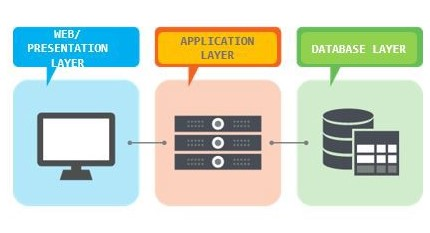
\includegraphics[width=5in]{images/threeTierArchitecture}
  \caption{The three-tier architecture}
  \label{threeTierArchitecture}
\end{figure}

The three-tier architecture represents the simplest layering scheme that could be successfully applied to an enterprise application. However, if the application is quite complex, it would indeed need additional mediating layers. This raises the question of how to further split the layers and how the dependencies between layers should be managed. The Software Engineering field has seen quite a few architecture models which serve exactly this purpose.

"The Clean Architecture" seen in Figure \ref{cleanArchitectureImg} is, as described in \cite{cleanArchitecture}, an attempt to integrate and combine several architectures having as end goal the separation of concerns, which results in modular systems composed of fairly independent components.

\begin{figure}[H]
  \centering
  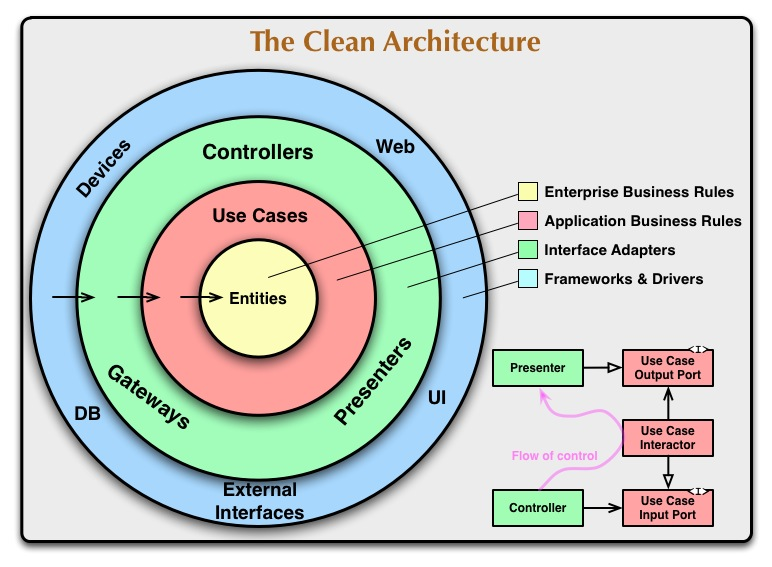
\includegraphics[width=6in]{images/cleanArchitecture}
  \caption{The clean architecture \cite{cleanArchitecture}}
  \label{cleanArchitectureImg}
\end{figure}

The circles in Figure \ref{cleanArchitectureImg} show different components of a software application:

\begin{itemize}
  \item \textbf{Entities} represent the business objects of the application.
  \item \textbf{Use cases} encapsulate the business logic and is not affected by changes to the database or the UI.
  \item \textbf{Interface adapters} act as converters between data formats and handle communication between use cases and entities with the database or the web GUI.
  \item \textbf{Frameworks and drivers} is a layer composed mainly of tools - be it the database or the web framework.
\end{itemize}

Of course, a really clean architecture would imply a low coupling of layers, that would permit the components to remain independent of one another. The business layer should be independent of the database, allowing it to be replaced with a different data source as long as the model objects keep the same structure. At the same time, it should also be independent of the UI. Thus, the UI could change, be redesigned or reimplemented using another framework without even touching the business layer. This separation also contributes to making the business layer highly testable on its own, without involving the actual database or the UI.

To achive this low coupling, an important rule must be kept in mind when defining dependencies between modules and layers. This is described in \cite{cleanArchitecture} as "The Dependency Rule", which states that "Source code dependencies must point only inward". To clarify this, let's look again at Figure \ref{cleanArchitectureImg}. According to the rule, components from an inner circle should not know about components from an outer circle. From a code perspective, this means that any software entity should use only those software entities that were declared in an inner circle. As an example, a controller, which belongs to the Interface Adapters group, cannot use an entity defined in the Web Presentation layer, which belongs to Frameworks and Drivers. Instead, it is the responsiblity of the Web Presentation layer to make a request to the controller, which will then invoke the Application layer and so on.

Building dependencies according to this rule will result in a layered design with a structure that resembles a \textit{directed acyclic graph} (DAG), meaning that it has no cycles. This will ensure that the components are independent of one another, which will make them easier to develop, maintain and extend.


\subsection{Client-server communication: Representational State Transfer}
\label{subsection:rest}

In the previous subsection, we have talked about the separation of client and server so that each of them could be individually developed and changed without affecting the other part. However, the only way to achieve this modularity is to establish a communication standard between the server and the client.

This could be accomplished by using Representational State Transfer (REST), which is an architectural style for providing standards for communication between web systems. It was designed as an alternative to Simple Object Access Protocol (SOAP), which has been, for a long time, the mainly used architectural style for building web services. However, due to its simplicity, lightweightness and scalability, REST has quickly gained popularity and is nowadays the most popular approach chosen for web service development.

The decoupling of the client and server is one of the 6 constraints of the REST architectural style. The communication is made via the defined Application Programming Interface (API) using requests and responses. Clients will send requests using the HTTP protocol and wait for responses. The server will receive those requests and do whatever the client needs, i.e. query the database or perform some other operations. When the REST service will finish processing the reuqest, it will send back a response to the client (See Figure \ref{rest}). It is worth mentioning that the communication is always initiated by the client. The server will never share information about its resources on its own: it will wait and only send responses as reactions to incoming requests.

\begin{figure}[H]
  \centering
  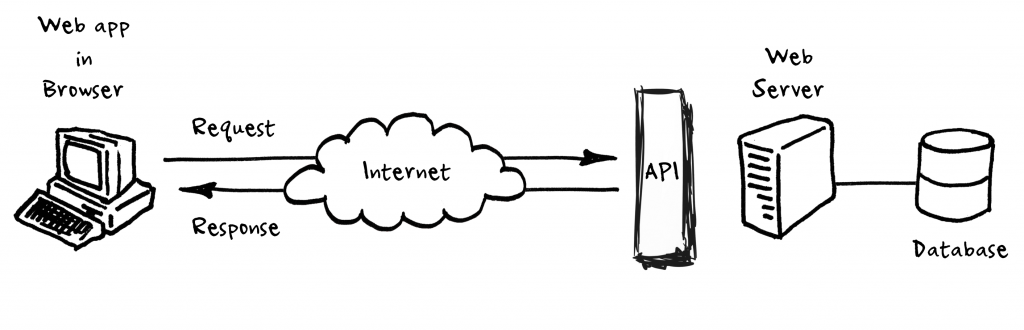
\includegraphics[width=5in]{images/rest}
  \caption{The client-server communication using a REST API \cite{rest}}
  \label{rest}
\end{figure}

What operation will be triggered on the server is determined by the information the client has to provide while making the request:

\begin{itemize}
  \item The \textbf{endpoint}, which is the Uniform Resource Identifier (URI) for the requested resource.
  \item The \textbf{HTTP method} that tells the server which operation needs to be performed on the resource. (See Table \ref{httpVerbs})
\end{itemize}

\begin{table}[H]
  \centering
  \begin{tabular}{|c|l|}
    \hline
    GET    & read a resource             \\ \hline
    POST   & create a new resource       \\ \hline
    PUT    & update an existing resource \\ \hline
    DELETE & delete a resource           \\ \hline
  \end{tabular}
  \caption{The basic HTTP verbs}
  \label{httpVerbs}
\end{table}

Another important REST constraint says that the client-server communication is \textbf{stateless}, meaning that each single client request should contain all the information that the server needs for processing. It does not store a history of the requests and thus cannot use some previous context. Session state management is therefore entirely the client's responsibility. This is one of the main reasons why RESTful web services are so lightweight, scalable and easy to implement.


\subsection{Usability in the context of Enterprise Application Design}
\label{subsection:usability}

We had already mentioned in the previous section that usability is an important ingredient for a successful application. Now is the time to analyze in more detail what usability means and how it should be achived in our application.

In regard to web applications and software applications in general, usability is defined as the ease at which an average person can use the software to benefit from its functionality. This includes a wide range of characteristics: how intuitive the UI is, how memorable the workflows are, how time-efficient each operation is, as well as how much satisfaction it brings to the user. In the context of enterprise applications all these seem especialy important, as tools made to improve efficiency become useless if they are not efficient to use.

It may seem at first sight that achieving usability is only a matter of design, a correct placement of widgets on a page and a tasteful combination of colors. However, usability is much more than that. Some decisions made to improve usability can even influence the backend implementation of the system. Consider for example the application which is the subject of this thesis. As one of its primary functions will be tracking all documents in the organization, it will have to display all the existing data, so the UI will most probably contain a table of some sort. What will start as a couple of documents to be displayed will quickly grow to be a large collection of data registered into the system. Yet displaying all the data on one single page will be hard to interpret for the human eye. A best practice for avoiding this is using pagination to split the documents into multiple pages, thus limiting the number of rows diplayed on a single page \cite{modernEnterpriseUiDesign}. This is exactly the case when for achieving a task which will improve usability, we will have to also change the backend implementation to support handling paginated requests.

Another way of dealing with a lot of data as an alternative to pagination is loading the next chunk of data when the user scrolls to the bottom of the screen. This, however, makes the user unaware of the total amount of data and provides less control over navigation between data rows. This makes it more suitable for apps with and endless stream of data that the user should consume, while pagination is more suitable for enterprise applications like ours.

Another thing to keep in mind is the responsiveness of the application. After the client sends a request, receiving a response will occur with a certain delay called \textbf{response time} - the time it will take the server to process the request. The amount of time needed will depend on the nature of the request, as well as the latency - the minimum delay that is present even when no processing from the server is required. While there are a number of things to be considered when implementing the application that could improve overall performance and minimize response time, you could also do something to improve the experience on the UI side. Improve \textbf{responsiveness}, which represents the time in which the system aknowledges the request. Responsiveness and response time are the same if during a request processing the system is waiting without any indicator to the user. However, adding a progress spinner will improve responsiveness as the user will be aware that the request is processing. This will improve the overall experience, even if the response time will be the same.



% - architecture/patterns
% - "It is not enough for code to work." Robert C. Martin, Clean Code: A Handbook of Agile Software Craftsmanship

